\subsection[L'overfitting]{L'overfitting}

\begin{frame}

	\frametitle{L'overfitting}

	\begin{columns}
			\column{0.55\linewidth}
%			Un semplice caso di overfitting: le linee verdi e nere rappresentano modelli di classificazione overfitting e non-overfitting. La linea verde classifica perfettamente i dati del training-set, ma sembra che sia troppo dipendente da quei dati (memorizzazione dei dati / memorizing the data).\\
%			È molto probabile che la linea verde abbia un tasso di errore più elevato sui nuovi dati non visualizzati, rispetto alla linea nera.

			Per sviluppare un po' di intuizione su questo concetto, guarderemo tre figure.
			\newlinedouble
			Supponiamo che ogni punto in queste figure rappresenti la posizione di un albero in una foresta.\\
			I due colori hanno i seguenti significati:
			\begin{itemize}
				\item punti blu: alberi malati
				\item punti rossi: alberi sani
			\end{itemize}

			\column{0.45\linewidth}
			\begin{figure}[!htbp]
				\centering
				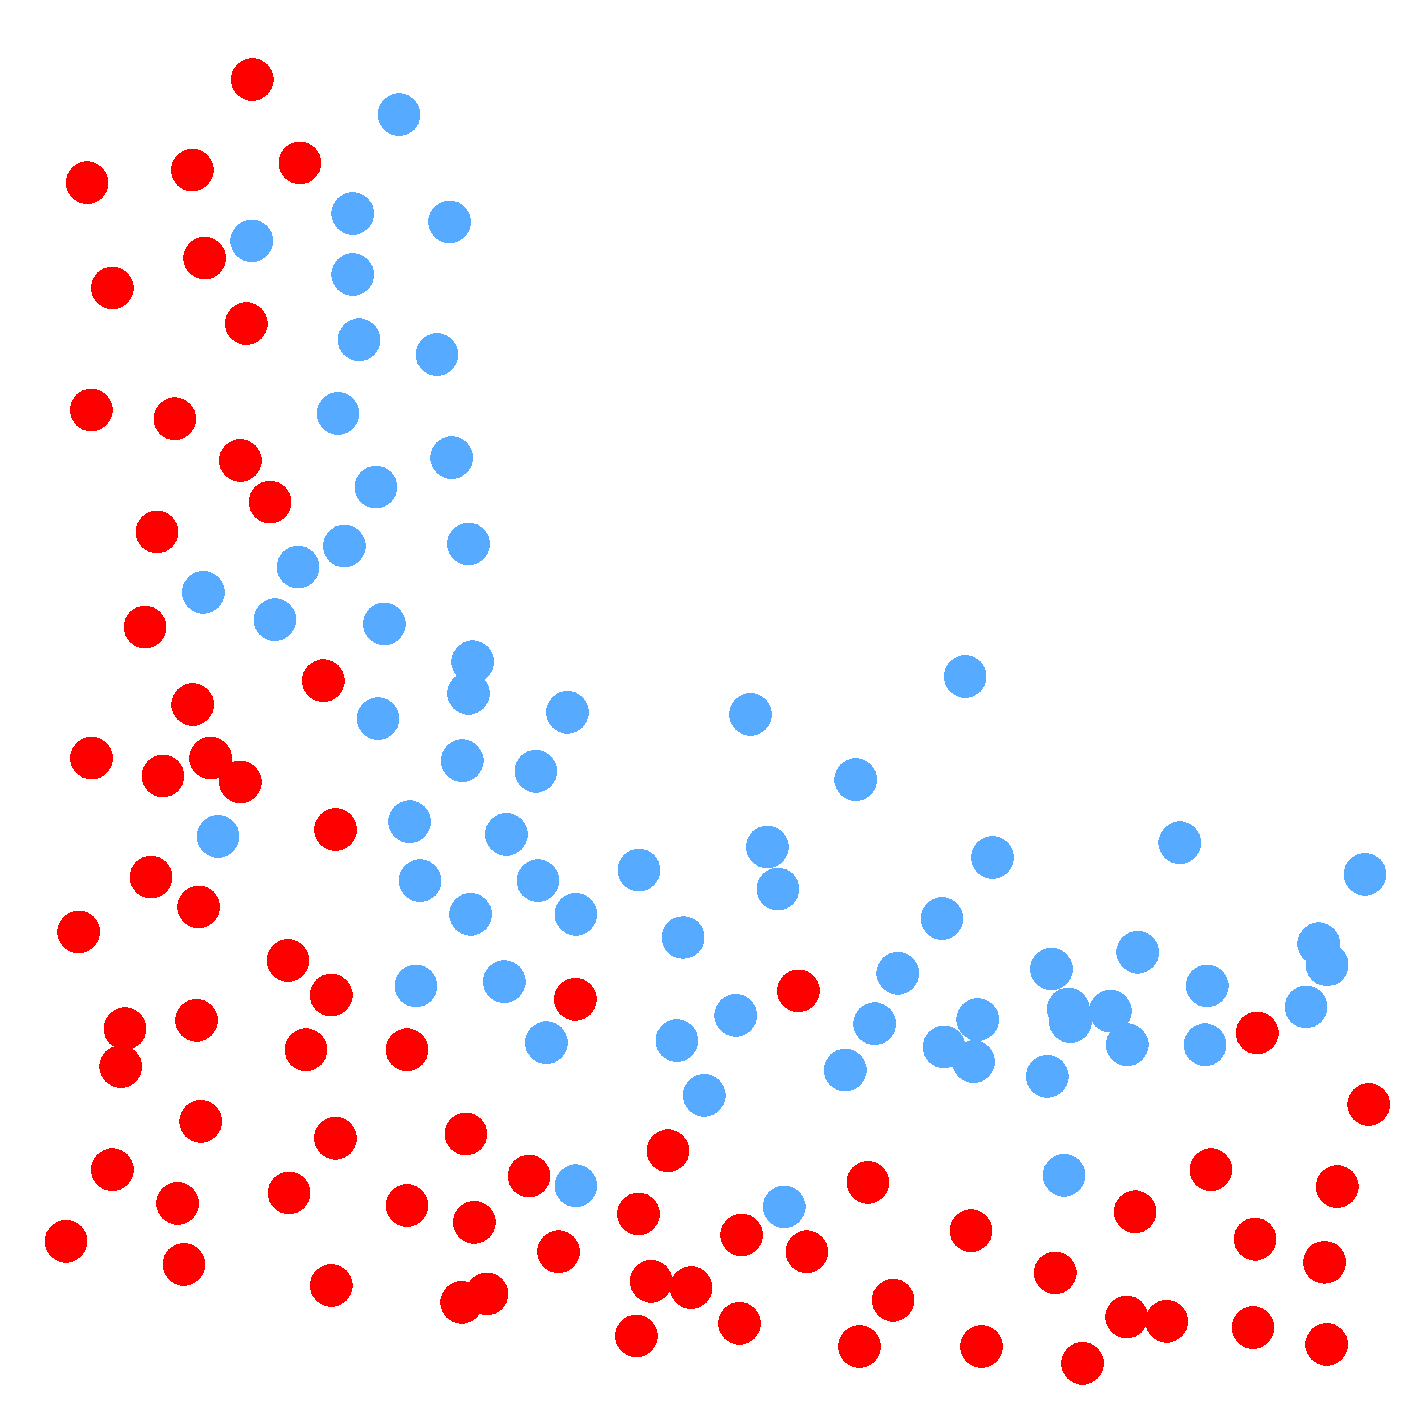
\includegraphics[width=1.0\linewidth]{images/supervised/validation_test_training_peril_of_overfitting/overfitting.pdf}
%				\caption{Alberi malati (in blu) e sani (in rosso)}
%				\label{}
			\end{figure}

	\end{columns}
\end{frame}

\begin{frame}

	\frametitle{L'overfitting}

	\begin{columns}
			\column{0.55\linewidth}
			Riuscite a immaginare un buon modello per prevedere i successivi alberi malati o sani?
			\newlinedouble
			Prenditi un momento per disegnare mentalmente un arco che divide il blu dalle arance, o mentalmente tracciare una linea che suddivida il gruppo blu da quello rosso.

			\column{0.45\linewidth}
			\begin{figure}[!htbp]
				\centering
				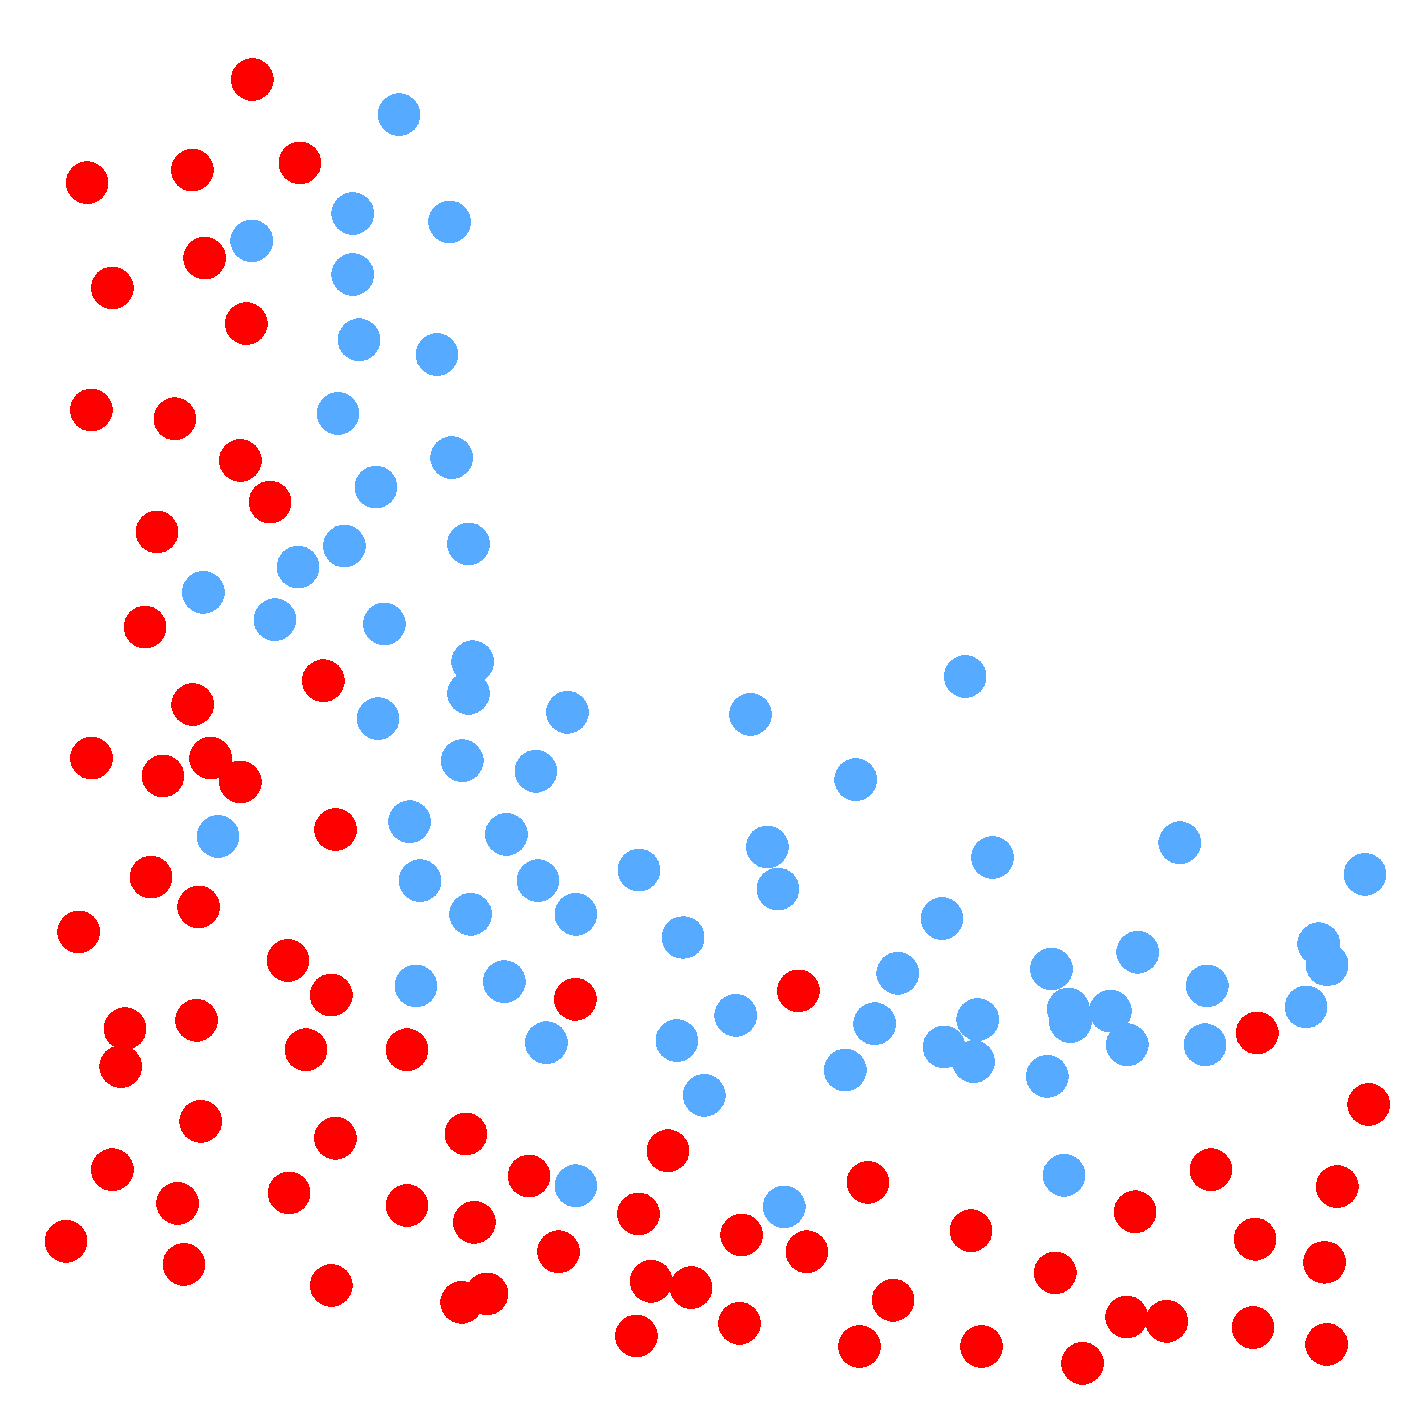
\includegraphics[width=1.0\linewidth]{images/supervised/validation_test_training_peril_of_overfitting/overfitting.pdf}
%				\caption{Alberi malati (in blu) e sani (in rosso)}
%				\label{}
			\end{figure}

	\end{columns}
\end{frame}


\begin{frame}

	\frametitle{L'overfitting}

	\begin{columns}
			\column{0.55\linewidth}
			In figura si mostra come un certo modello di apprendimento automatico molto flessibile possa separare perfettamente gli alberi malati da quelli sani.\\
			Si noti che questo modello ha prodotto una perdita molto molto bassa.
			\newlinedouble
			A prima vista, il modello mostrato in figura sembra fare un ottimo lavoro nel separare gli alberi sani da quelli malati.


			\column{0.45\linewidth}
			\begin{figure}[!htbp]
				\centering
				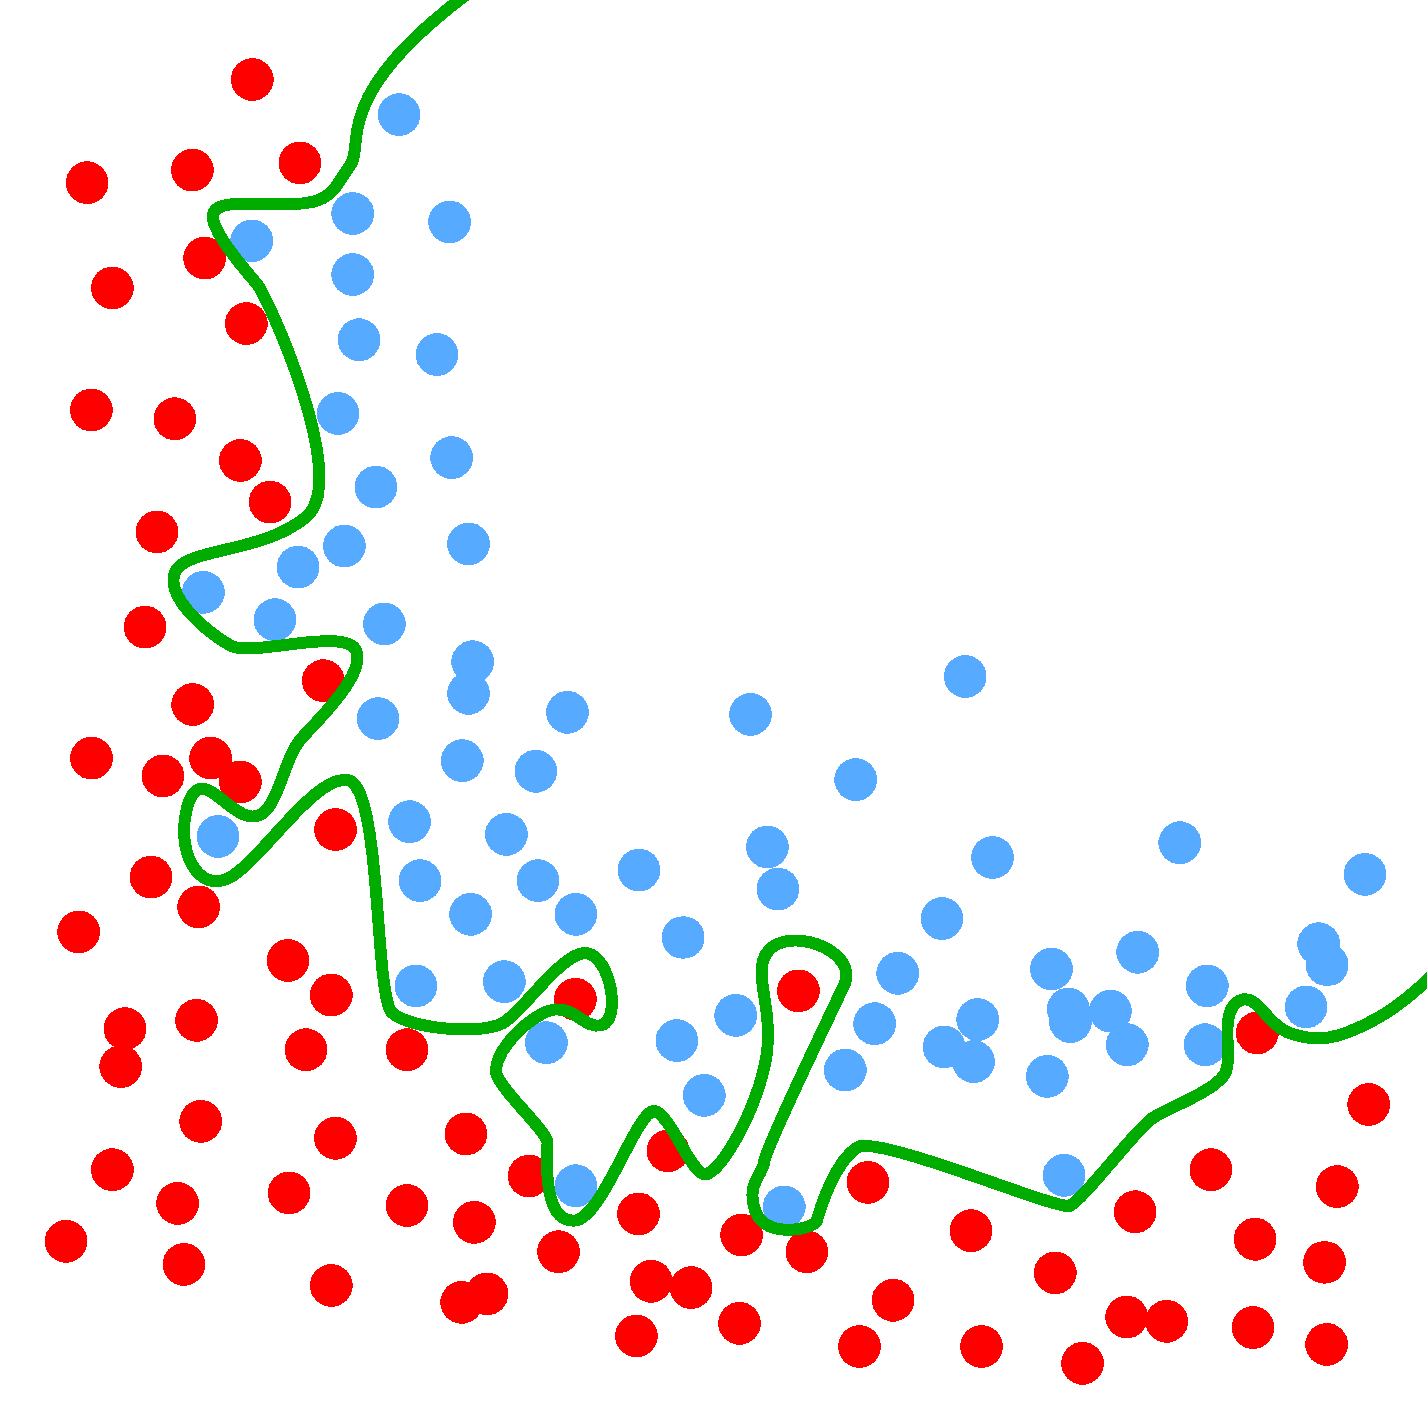
\includegraphics[width=1.0\linewidth]{images/supervised/validation_test_training_peril_of_overfitting/overfitting_green_line.pdf}
%				\caption{Alberi malati (in blu) e sani (in rosso)}
%				\label{}
			\end{figure}

	\end{columns}
\end{frame}


\begin{frame}

	\frametitle{L'overfitting}
 
	\begin{columns}
			\column{0.55\linewidth}
			A prima vista, il modello mostrato nella in figura sembra\textbf{VA} fare un ottimo lavoro nel separare gli alberi sani da quelli malati!
			\newlinedouble
			Infatti la nuova figura mostra cosa è successo quando abbiamo aggiunto dei nuovi dati al grafico.\\

			In blu e rosso scuro non indicati i nuovi dati (appartenenti rispettivamente ad alberi malati ed alberi sani).\\

			Si è scoperto quindi che il modello in realtà si adatta molto male ai nuovi dati.\\
			Si noti che il modello ha classificato in modo errato una buona parte dei nuovi dati.



			\column{0.45\linewidth}
			\begin{figure}[!htbp]
				\centering
				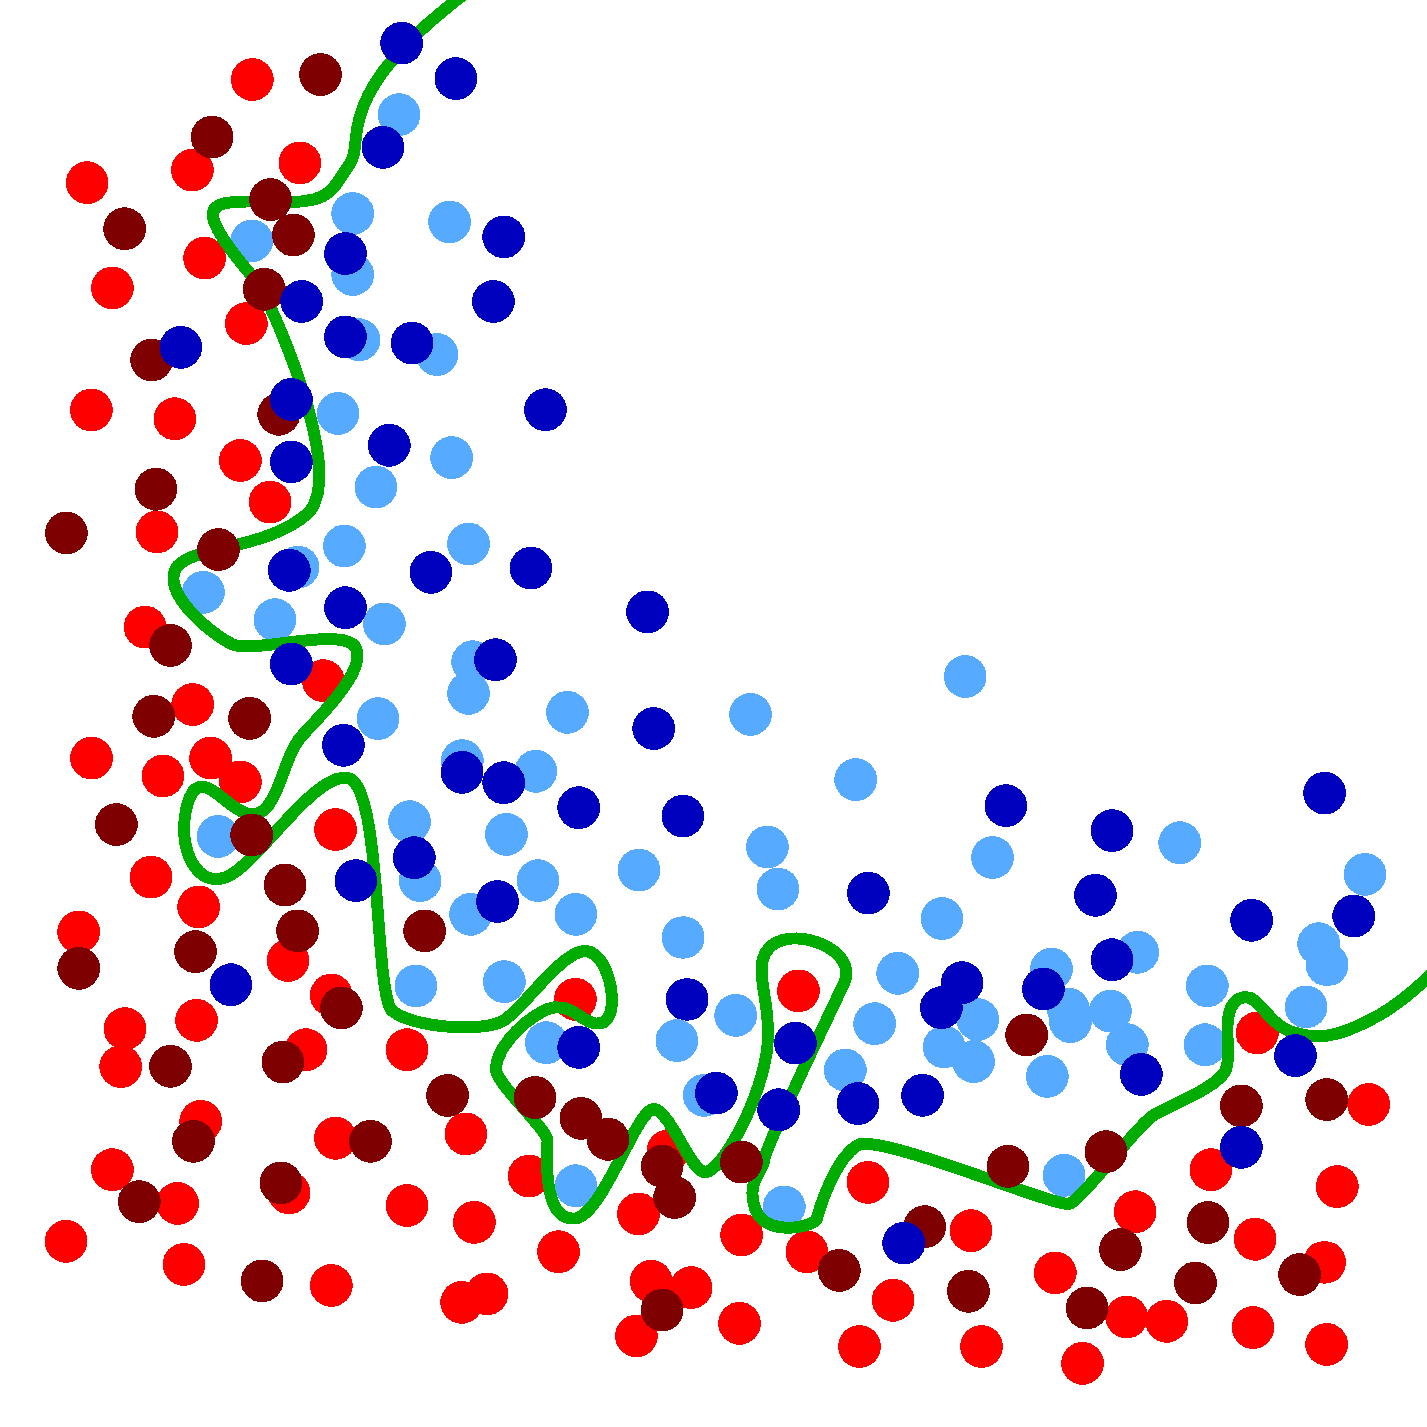
\includegraphics[width=1.0\linewidth]{images/supervised/validation_test_training_peril_of_overfitting/overfitting_green_line_with_test.pdf}
%				\caption{Alberi malati (in blu) e sani (in rosso)}
%				\label{}
			\end{figure}

	\end{columns}
\end{frame}


\begin{frame}

	\frametitle{L'overfitting}

	\begin{columns}
			\column{0.55\linewidth}
			Il modello mostrato overfitta le peculiarità dei dati su cui si è addestrato.\\
			È un po' come preparare degli studenti sempre su degli esercizi di matematica molto complicati e poi stimare la loro bravura con dei compiti solo su quegli esercizi.
			\newlinedouble
			Un modello che subisce overfitting ha una bassa loss durante l'allenamento, ma non riesce a fare previsioni molto corrette con dei nuovi dati.\\
			Se un modello si adatta bene al campione attuale, come possiamo fidarci che farà buone previsioni su nuovi dati?

			\column{0.45\linewidth}
			\begin{figure}[!htbp]
				\centering
				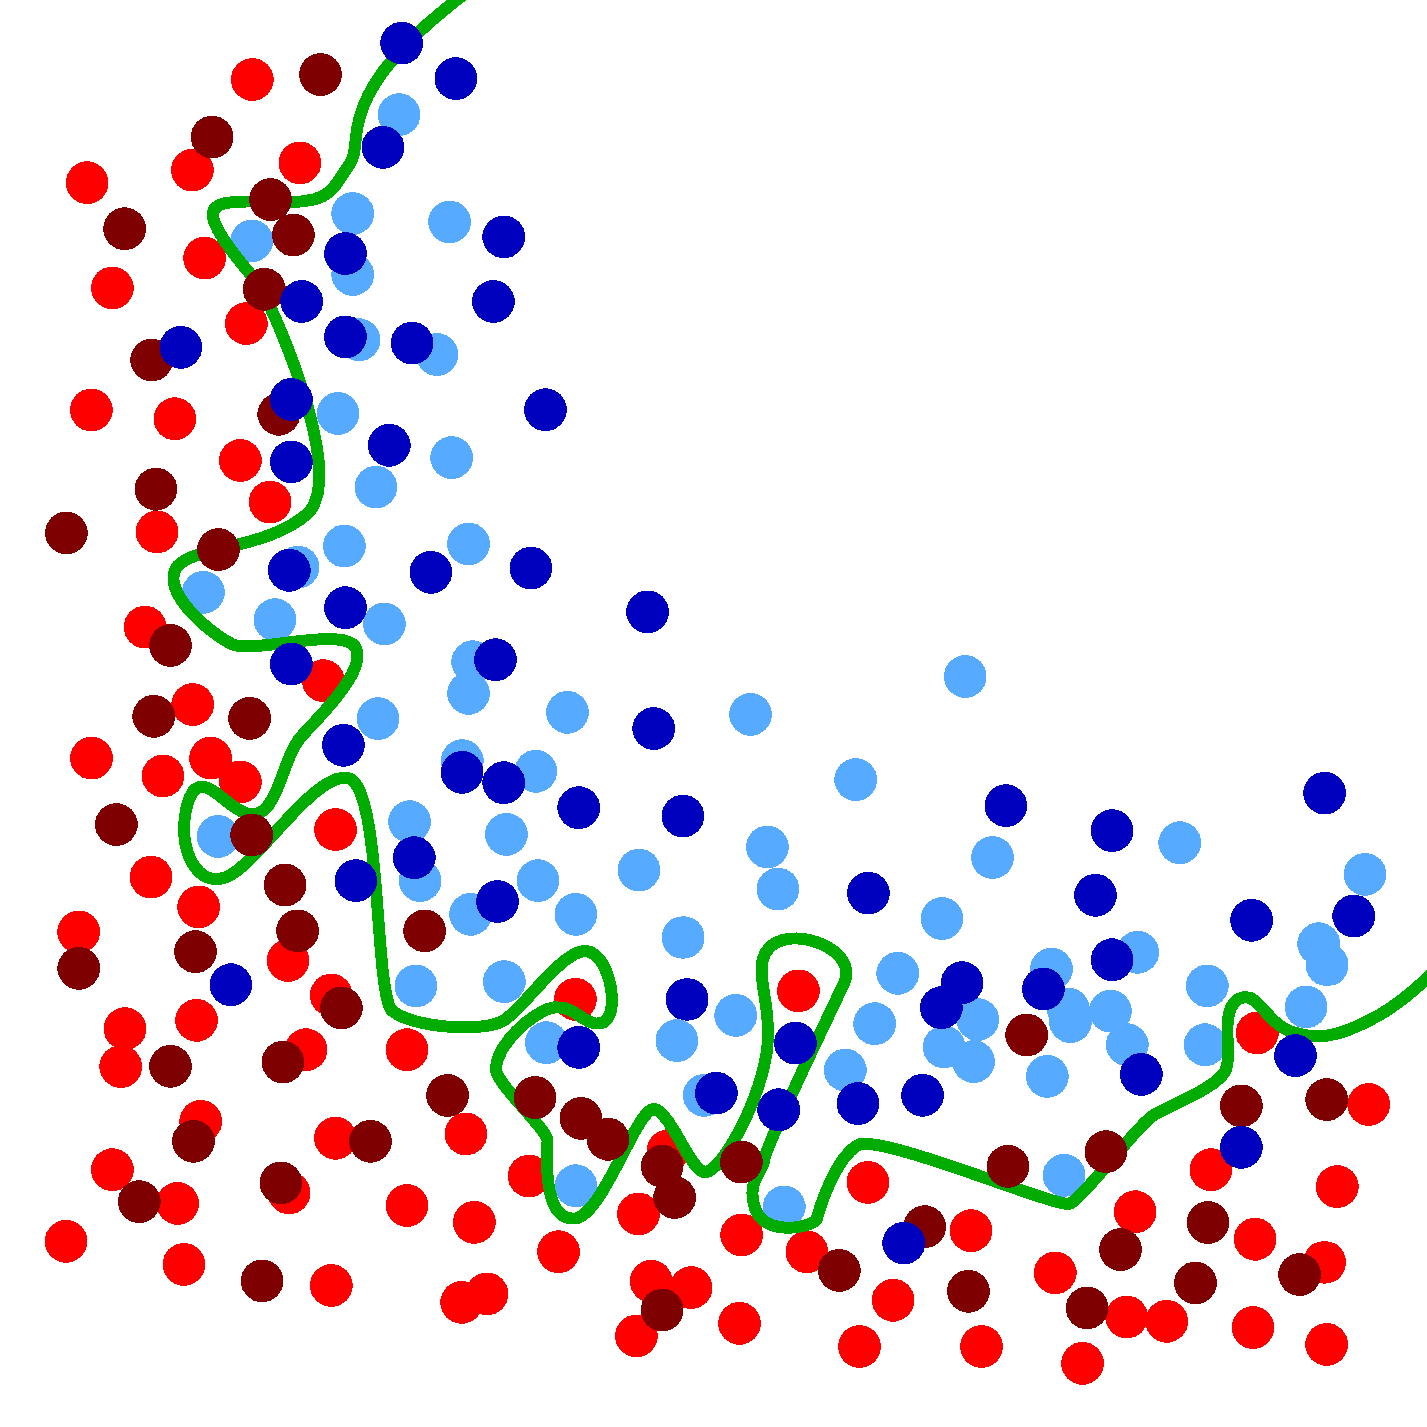
\includegraphics[width=1.0\linewidth]{images/supervised/validation_test_training_peril_of_overfitting/overfitting_green_line_with_test.pdf}
%				\caption{Alberi malati (in blu) e sani (in rosso)}
%				\label{}
			\end{figure}

	\end{columns}
\end{frame}


\begin{frame}

	\frametitle{L'overfitting}

	\begin{columns}
			\column{0.55\linewidth}
			L'overfitting è principalmente causato dall'addestrare un modello più complesso del necessario.
			\newlinedouble
			Lo scopo fondamentale dell'apprendimento automatico è trovare un trade-off tra l'adattamento ai dati e la semplicità del modello.
			\newlinedouble
			In nero viene mostrato un possibile modello meno flessibile (e quindi anche più semplice) ma più efficace del precedente.
			\column{0.45\linewidth}
			\begin{figure}[!htbp]
				\centering
				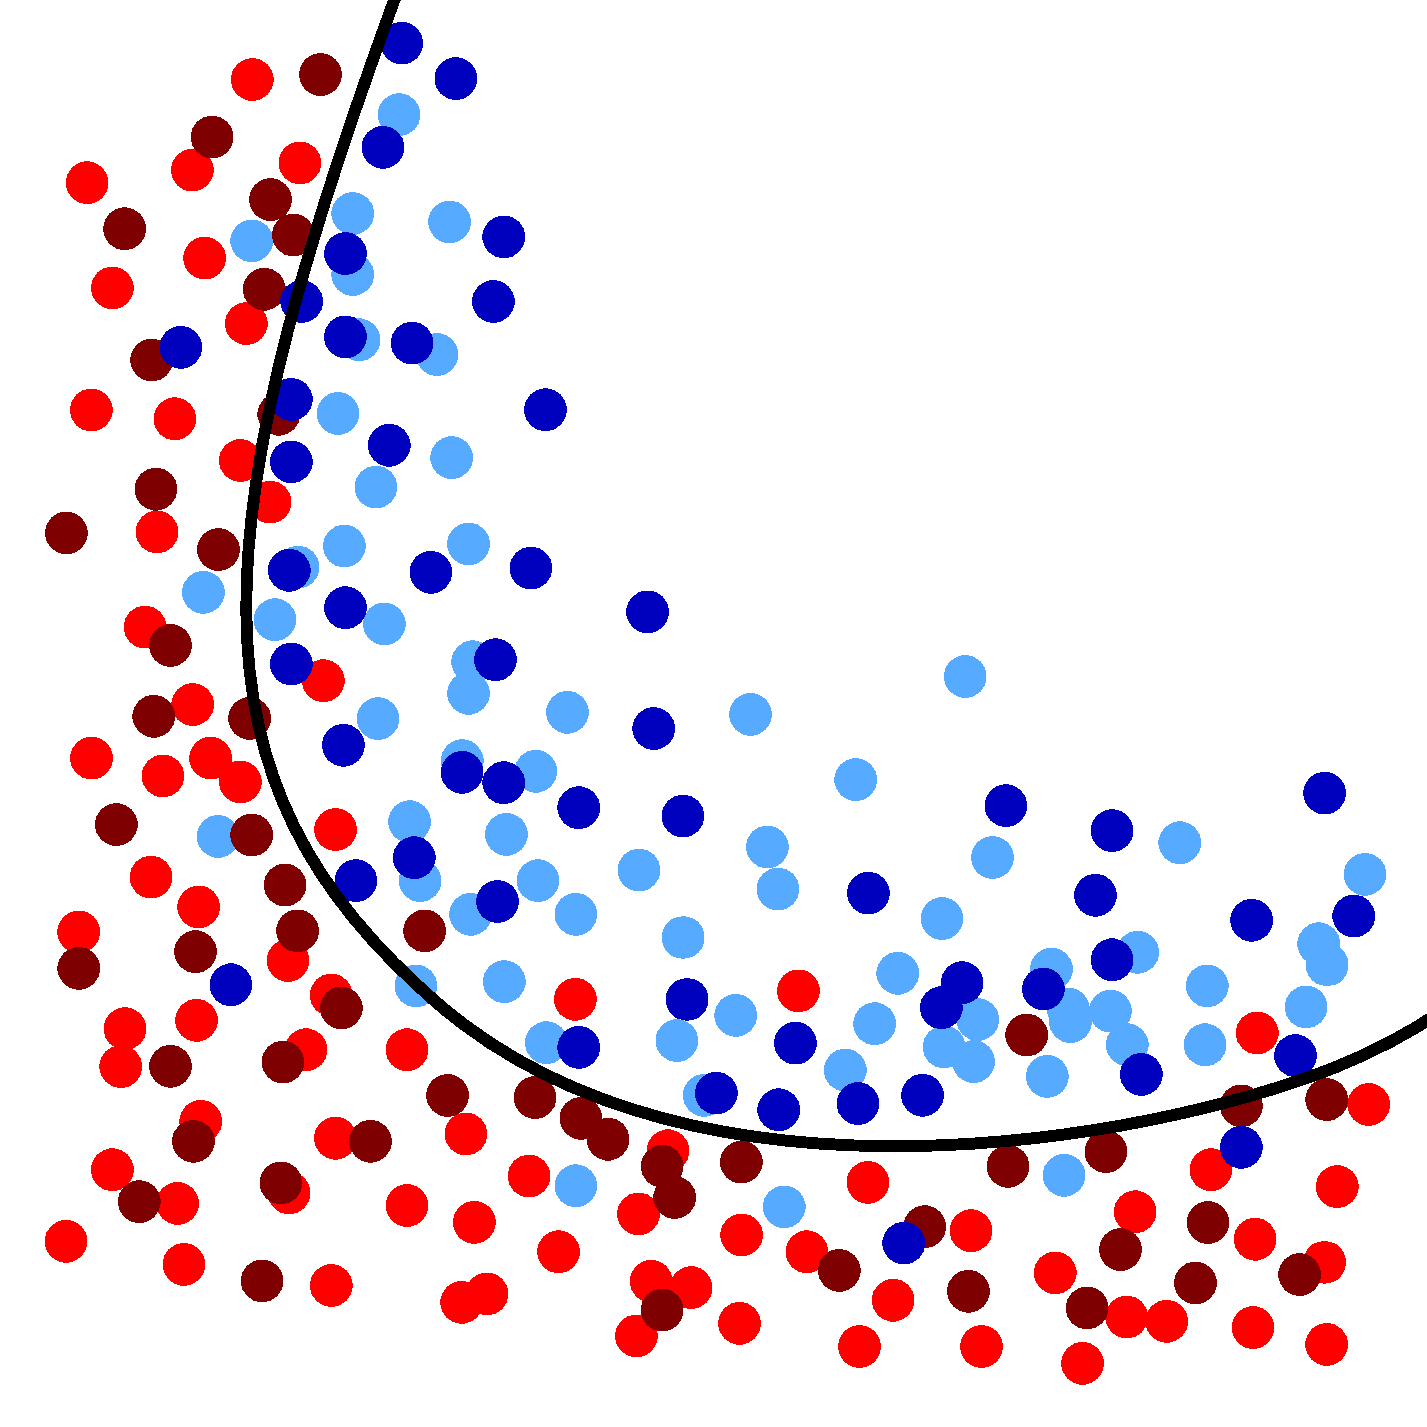
\includegraphics[width=1.0\linewidth]{images/supervised/validation_test_training_peril_of_overfitting/overfitting_black_line_with_test.pdf}
%				\caption{Alberi malati (in blu) e sani (in rosso)}
%				\label{}
			\end{figure}

	\end{columns}
\end{frame}


\begin{frame}

	\frametitle{L'overfitting}

	\begin{columns}
			\column{0.55\linewidth}
			L'obiettivo dell'apprendimento automatico è prevedere bene i nuovi dati tratti da una distribuzione di probabilità reale (nascosta).
			\newlinedouble
			Sfortunatamente, il modello non può vedere tutta la verità; il modello può campionare solo da un set di dati del training-set.
			\newlinedouble
			Se un modello si adatta bene agli esempi attuali, come puoi fidarti che il modello farà anche buone previsioni su esempi mai visti prima?

			\column{0.45\linewidth}
			\begin{figure}[!htbp]
				\centering
				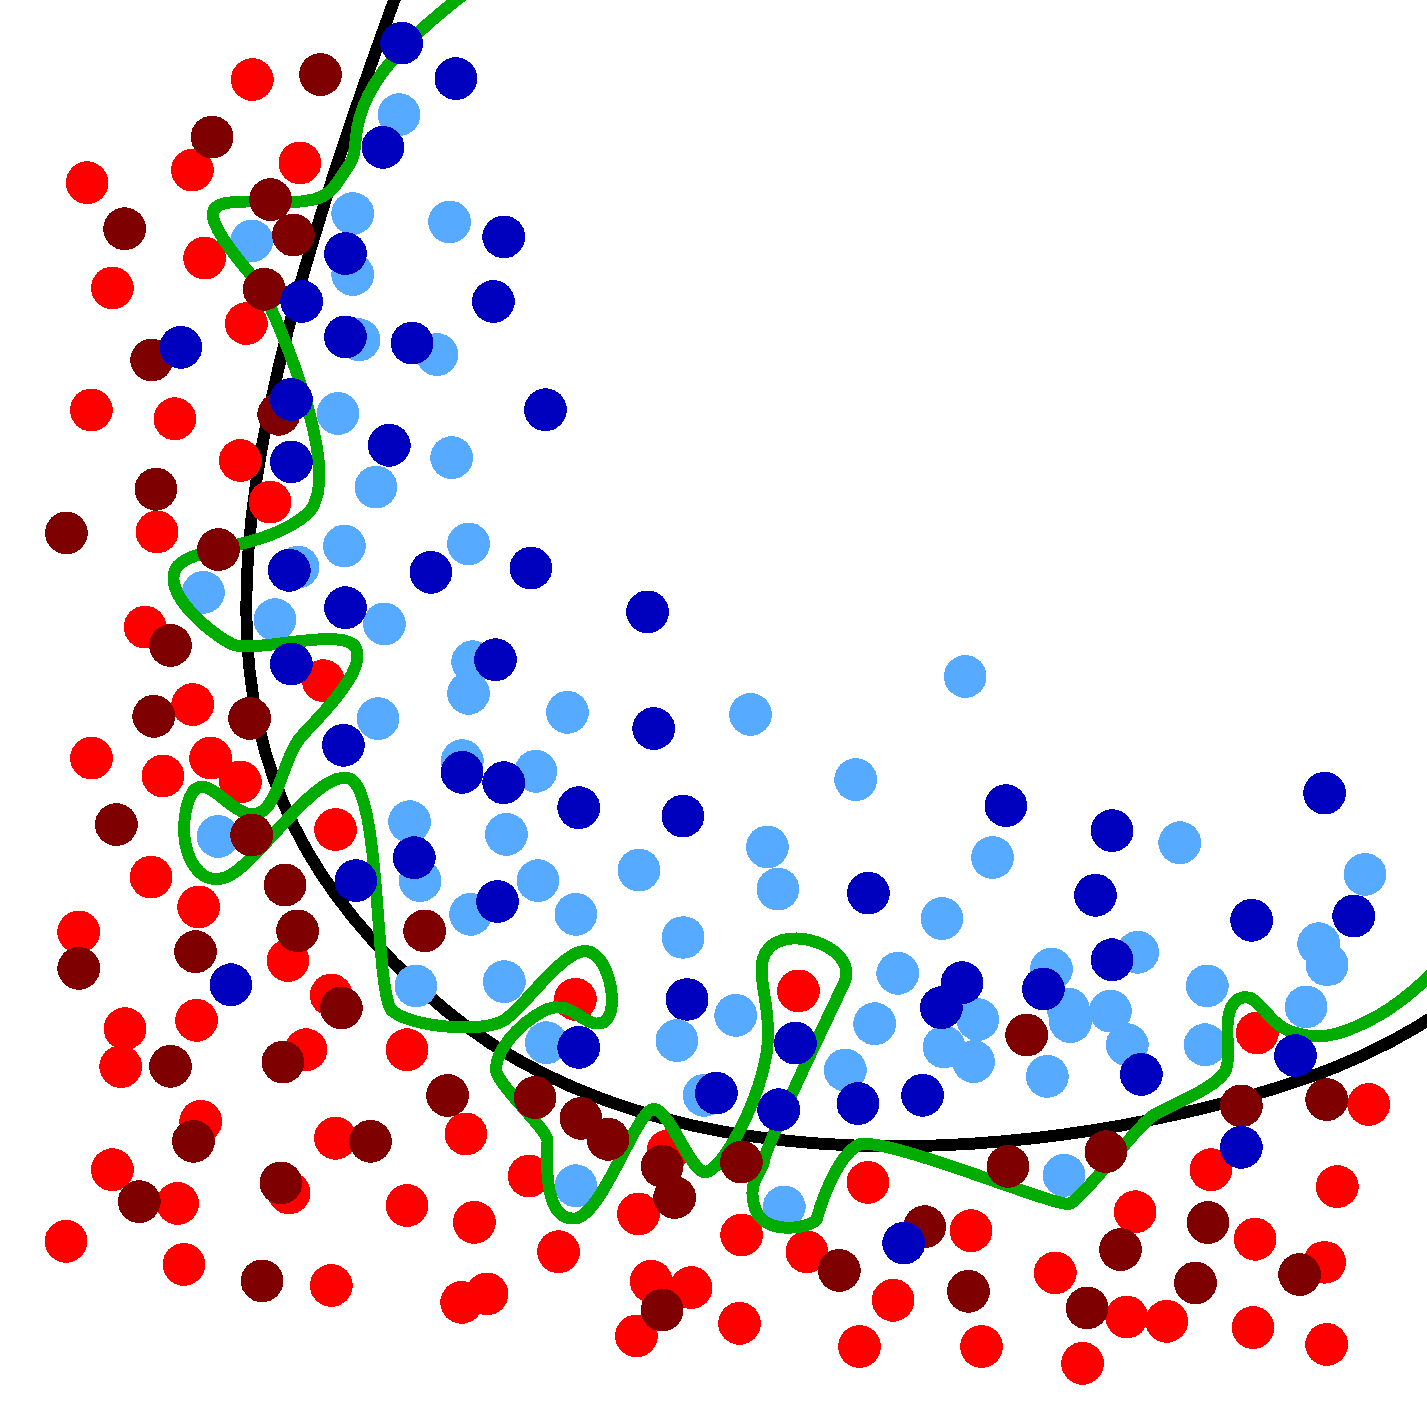
\includegraphics[width=1.0\linewidth]{images/supervised/validation_test_training_peril_of_overfitting/overfitting_black_green_lines_with_test.pdf}
%				\caption{Alberi malati (in blu) e sani (in rosso)}
%				\label{}
			\end{figure}

	\end{columns}
\end{frame}


\begin{frame}

	\frametitle{Il rasoio di Occam}

	\textbf{Guglielmo da Occam} (o da Ockham), un frate e filosofo del XIV secolo, amava la semplicità. Credeva che gli scienziati dovessero preferire formule o teorie più semplici a quelle più complesse.
	\newlinedouble
	Per mettere il rasoio di Occam nei termini del machine learning:\\
	meno complesso è un modello di ML, più è probabile che un buon risultato empirico non sia dovuto solo alle peculiarità del campione.
	\newlinedouble
	%In tempi moderni, abbiamo formalizzato il rasoio di Occam nei campi della teoria dell'apprendimento statistico e della teoria dell'apprendimento computazionale.
	%\newlinedouble
	\pause
	Una descrizione statistica della capacità di un modello nel generalizzare, utilizzando nuovi dati, può essere ottenuta soprattutto misurando:
	\begin{itemize}
		\item la complessità del modello
		\item le prestazioni del modello sul training-set
	\end{itemize}

\end{frame}


% valutare se ripristinare questa slide
%\begin{frame}
%
%	\frametitle{Assunzioni per una corretta generalizzazione}
%
%	I seguenti tre assunti di base guidano la generalizzazione:
%	\begin{itemize}
%		\item estraiamo esempi in modo indipendente e identico (i.i.d) in modo randomico dalla distribuzione
%		\item la distribuzione è stazionaria; ovvero la distribuzione non cambia all'interno del dataset
%		\item estraiamo esempi da partizioni della stessa distribuzione
%	\end{itemize}
%	\ \\
%	In pratica, a volte violiamo questi presupposti.
%	\newlinedouble
%	%Ad esempio: considera un modello che sceglie gli annunci da visualizzare.\\
%	%L'i.i.d. presupposto verrebbe violato se il modello basasse la sua scelta di annunci, in parte, su quali annunci l'utente ha visto in precedenza.
%	Consideriamo un set di dati che contiene informazioni sulle vendite al dettaglio per un anno. Gli acquisti dell'utente cambiano stagionalmente, il che viola la stazionarietà.\\
%	%\newlinedouble
%	Quando sappiamo che uno dei tre presupposti di base precedenti è stato violato, dobbiamo prestare \textbf{molta attenzione alle metriche}.
%
%\end{frame}
